% GearGuard - manuscript draft (IEEE conference format).
%
% STATUS: DRAFT. Everything marked \todo{...} needs real data before submission.
% Nothing in this file claims detector accuracy or user-study results: the app
% currently ships with a *simulated* detector (see Section IV-C), and no
% user study has been run yet.
%
% Build:  pdflatex main && bibtex main && pdflatex main && pdflatex main
\documentclass[conference]{IEEEtran}
\usepackage{cite}
\usepackage{amsmath,amssymb}
\usepackage{graphicx}
\usepackage{booktabs}
\usepackage{xcolor}
\usepackage{url}
\usepackage{listings}
\lstset{basicstyle=\ttfamily\footnotesize,breaklines=true,frame=single}
\newcommand{\todo}[1]{\textcolor{red}{\textbf{[TODO: #1]}}}
\graphicspath{{../screenshots/}}

\begin{document}

\title{GearGuard: A Detector-Agnostic Mobile Architecture for\\
Personal Protective Equipment Compliance Monitoring}

\author{\IEEEauthorblockN{Author Name}
\IEEEauthorblockA{Department, Institution\\
City, Country\\
email@example.com}}

\maketitle

\begin{abstract}
Verifying that workers wear the required personal protective equipment (PPE)
before entering a work area is a routine but error-prone safety task. Existing
research focuses mostly on the detection model, while the surrounding
workflow---identifying the worker, applying site-specific rules, recording the
result, and producing audit evidence---receives little attention. This paper
presents GearGuard, a cross-platform mobile application that covers that
workflow end to end. We contribute (i) a formal definition of per-scan and
per-worker compliance that is independent of any particular detector, (ii) a
detector-agnostic architecture in which a single interface isolates the machine
learning model from the user interface, storage and reporting layers, and
(iii) an open-source reference implementation in Flutter with scan, attendance,
ranking, archive and PDF-report features. The implementation is covered by unit
and end-to-end widget tests. \todo{Add one sentence with the headline result of
the detector benchmark and the usability study once they are run.}
\end{abstract}

\begin{IEEEkeywords}
personal protective equipment, occupational safety, mobile application,
object detection, software architecture, Flutter
\end{IEEEkeywords}

\section{Introduction}
Construction, manufacturing and logistics sites require workers to wear
helmets, high-visibility vests, gloves and safety footwear. Compliance is
usually checked by a supervisor at the gate, which is slow, inconsistent and
leaves no structured record. Vision-based PPE detection has been studied
extensively~\cite{nath2020}, building on real-time detectors such as
YOLO~\cite{redmon2016}. However, a detector alone does not make a usable safety
tool: supervisors also need to know \emph{who} was scanned, \emph{which} rules
applied, and to retrieve the history for audits.

This paper makes three contributions:
\begin{enumerate}
  \item A detector-independent formalisation of compliance (Section~III).
  \item A layered architecture that treats the detector as a replaceable
        component behind one interface (Section~IV).
  \item An open-source implementation and its verification (Sections~V--VI).
\end{enumerate}
\todo{Add 3--5 sentences positioning the work against recent PPE-detection and
safety-management-app literature; verify every citation.}

\section{Related Work}
\todo{Survey (a) PPE detection with deep learning on construction and industrial
sites, (b) mobile or edge deployment of detectors, (c) digital safety
management and attendance systems. Cite peer-reviewed sources only and state the
gap: end-to-end workflow with a swappable detector.}

\section{Problem Formulation}
Let $\mathcal{P}$ be the set of supported PPE item types (helmet, vest, gloves,
boots, goggles, mask). A site configuration fixes a required subset
$R \subseteq \mathcal{P}$, $R \neq \emptyset$, and a confidence threshold
$\tau \in [0,1]$. For a frame, a detector returns a confidence
$c_p \in [0,1]$ for every $p \in \mathcal{P}$. An item is \emph{detected} when
$c_p \ge \tau$. The set of missing items is
\begin{equation}
M = \{\, p \in R \mid c_p < \tau \,\}.
\end{equation}
A scan is \emph{compliant} iff $M=\emptyset$, and its \emph{score} is
\begin{equation}
s = \frac{|R| - |M|}{|R|}.
\end{equation}
For a worker $w$ with scan set $S_w$, the compliance rate is
\begin{equation}
C_w = \frac{|\{\, x \in S_w \mid M_x=\emptyset \,\}|}{|S_w|},
\end{equation}
and workers are ranked by $C_w$ in descending order, breaking ties by the mean
score $\bar{s}_w$. The daily site rate is the same ratio taken over all scans
recorded on that day. $R$ and $\tau$ are stored with each scan, so historical
results remain valid when the site rules change later.

\section{System Design}
\subsection{Layered Architecture}
GearGuard is organised in four layers (Fig.~\ref{fig:arch}): \emph{domain}
(pure Dart value types: \texttt{PpeItem}, \texttt{Employee},
\texttt{ScanRecord}), \emph{data} (detector, storage, PDF builder),
\emph{state} (\texttt{flutter\_bloc} cubits with immutable states) and
\emph{presentation} (feature modules). Derived quantities such as $C_w$,
rankings and most-missed equipment are computed in the state layer rather than
in widgets, which keeps them unit-testable.

\begin{figure}[t]
\centering
\begin{lstlisting}
presentation  dashboard | scanner | attendance
              team | archive | settings
state         SafetyCubit | SettingsCubit
data          PpeDetector | SafetyRepository
              | report_pdf
domain        PpeItem | Employee | ScanRecord
\end{lstlisting}
\caption{Layers of the reference implementation. Dependencies point downward.}
\label{fig:arch}
\end{figure}

\subsection{Detector Interface}
The only contract between the model and the rest of the app is:
\begin{lstlisting}[language=Java]
abstract interface class PpeDetector {
  Future<Map<PpeItem, double>> detect();
}
\end{lstlisting}
It is injected at the application root, so replacing the simulated detector
with an on-device model (e.g., a YOLO network invoked through a platform
channel) requires no change to any screen, cubit or report.

\subsection{Interaction Design}
The bottom navigation exposes the five daily tasks (Home, Attendance, Scan,
Team, Archive). Design decisions include: violations sorted first in the
attendance list; a one-tap ``Scan'' action for workers who have not yet checked
in; a per-item confidence checklist with bounding-box overlay on the scan
result (Fig.~\ref{fig:scan}); and status that is never conveyed by colour alone
(every status pill carries an icon and text). Light and dark themes are
provided.

\begin{figure}[t]
\centering
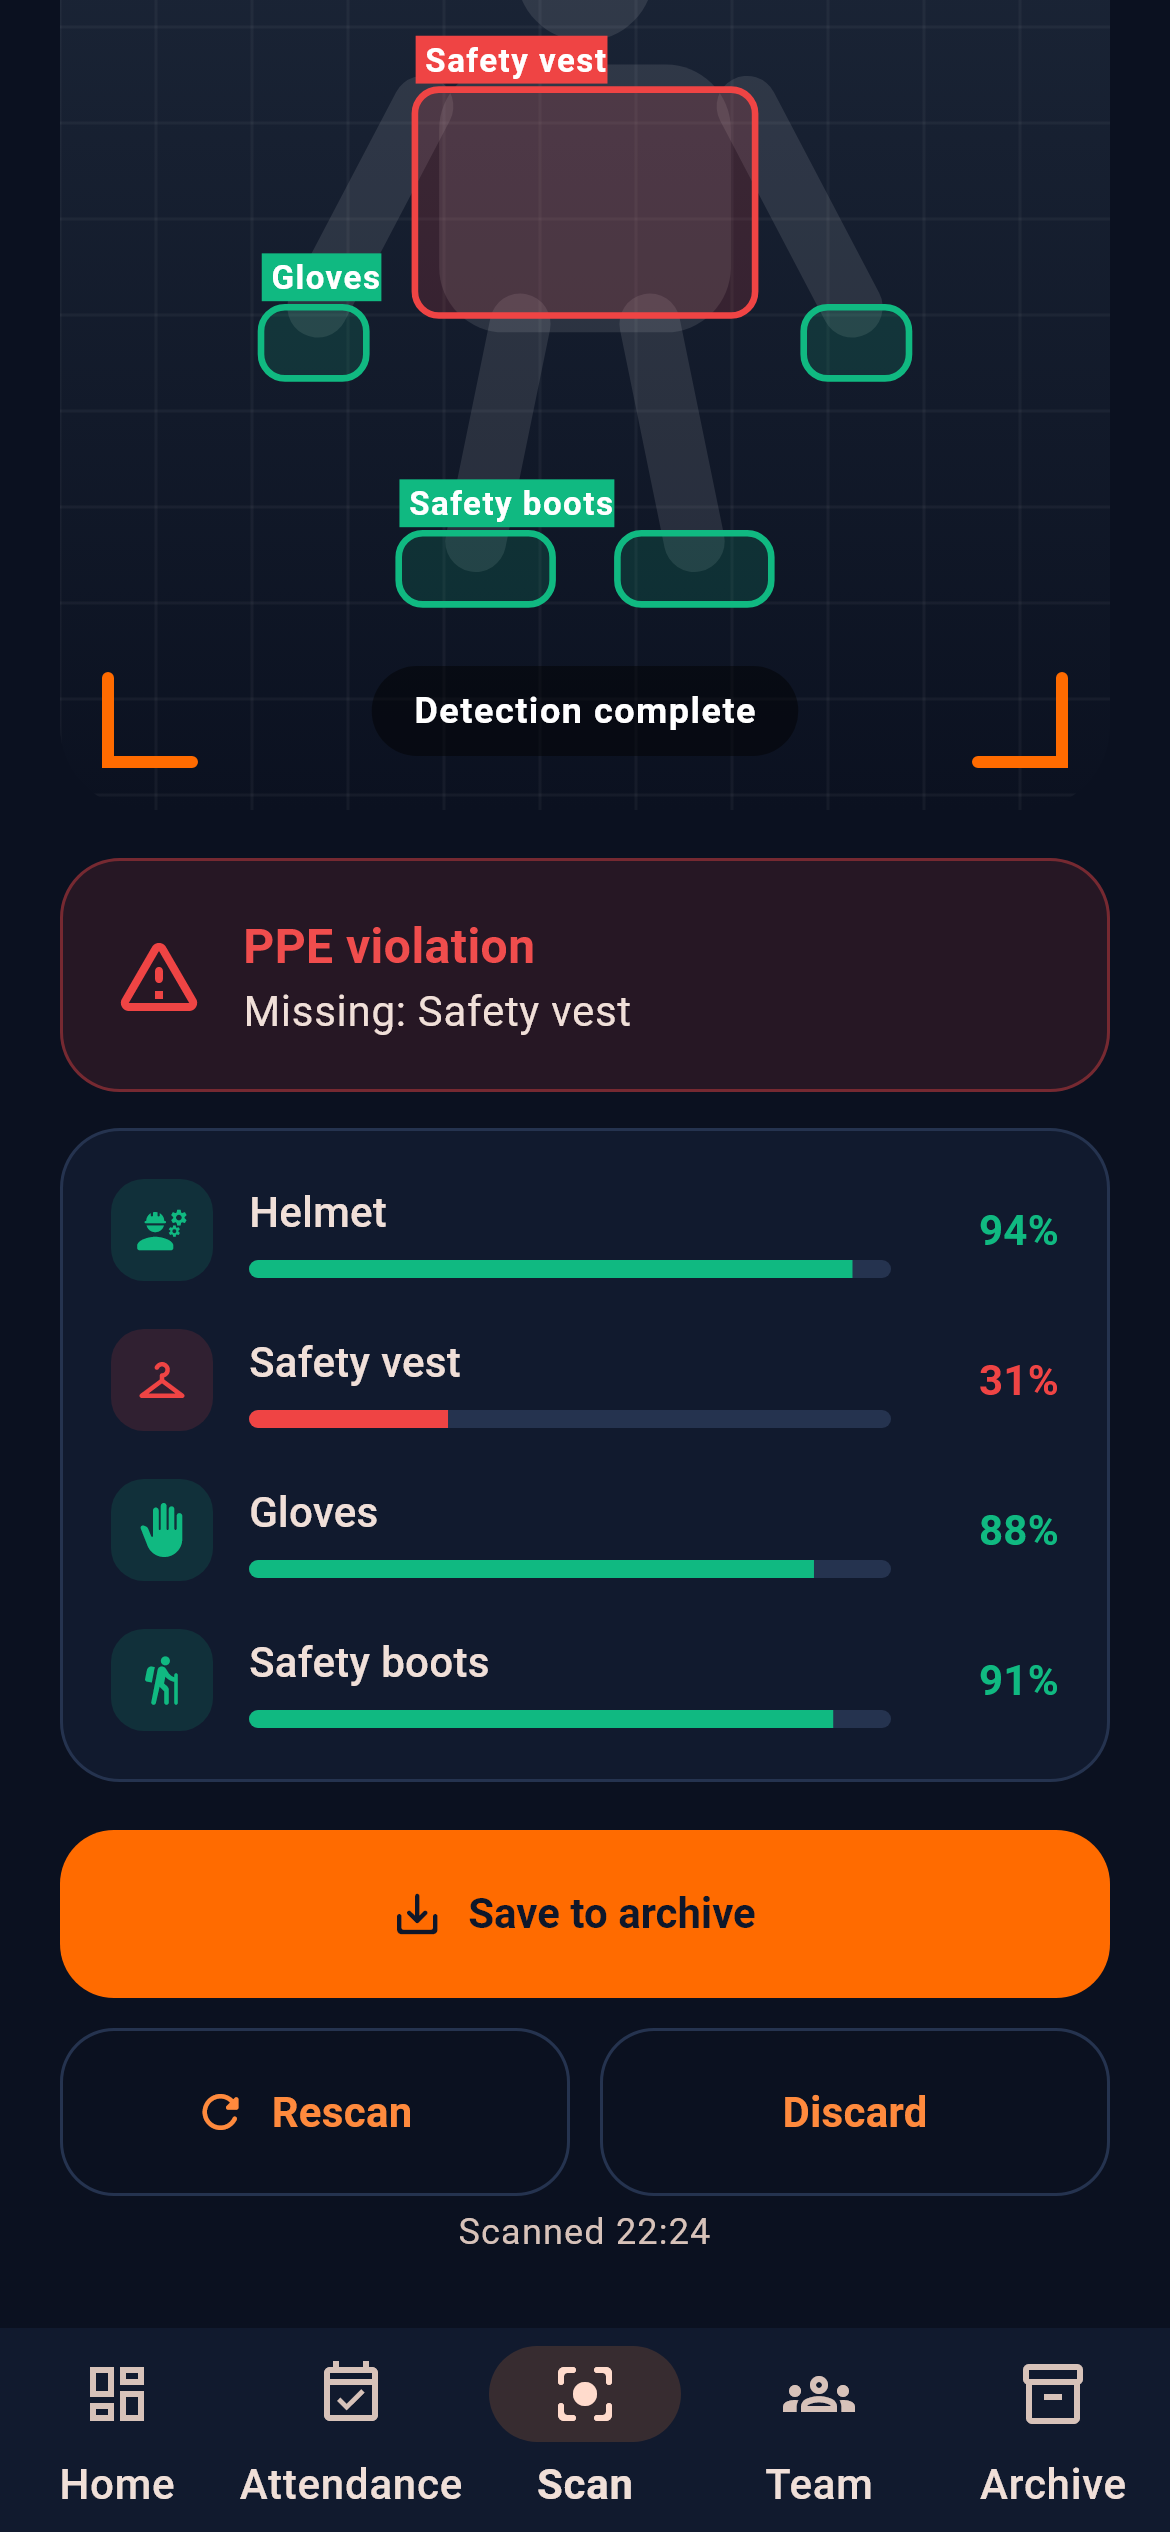
\includegraphics[width=0.42\columnwidth]{04-scan-result.png}\hfill
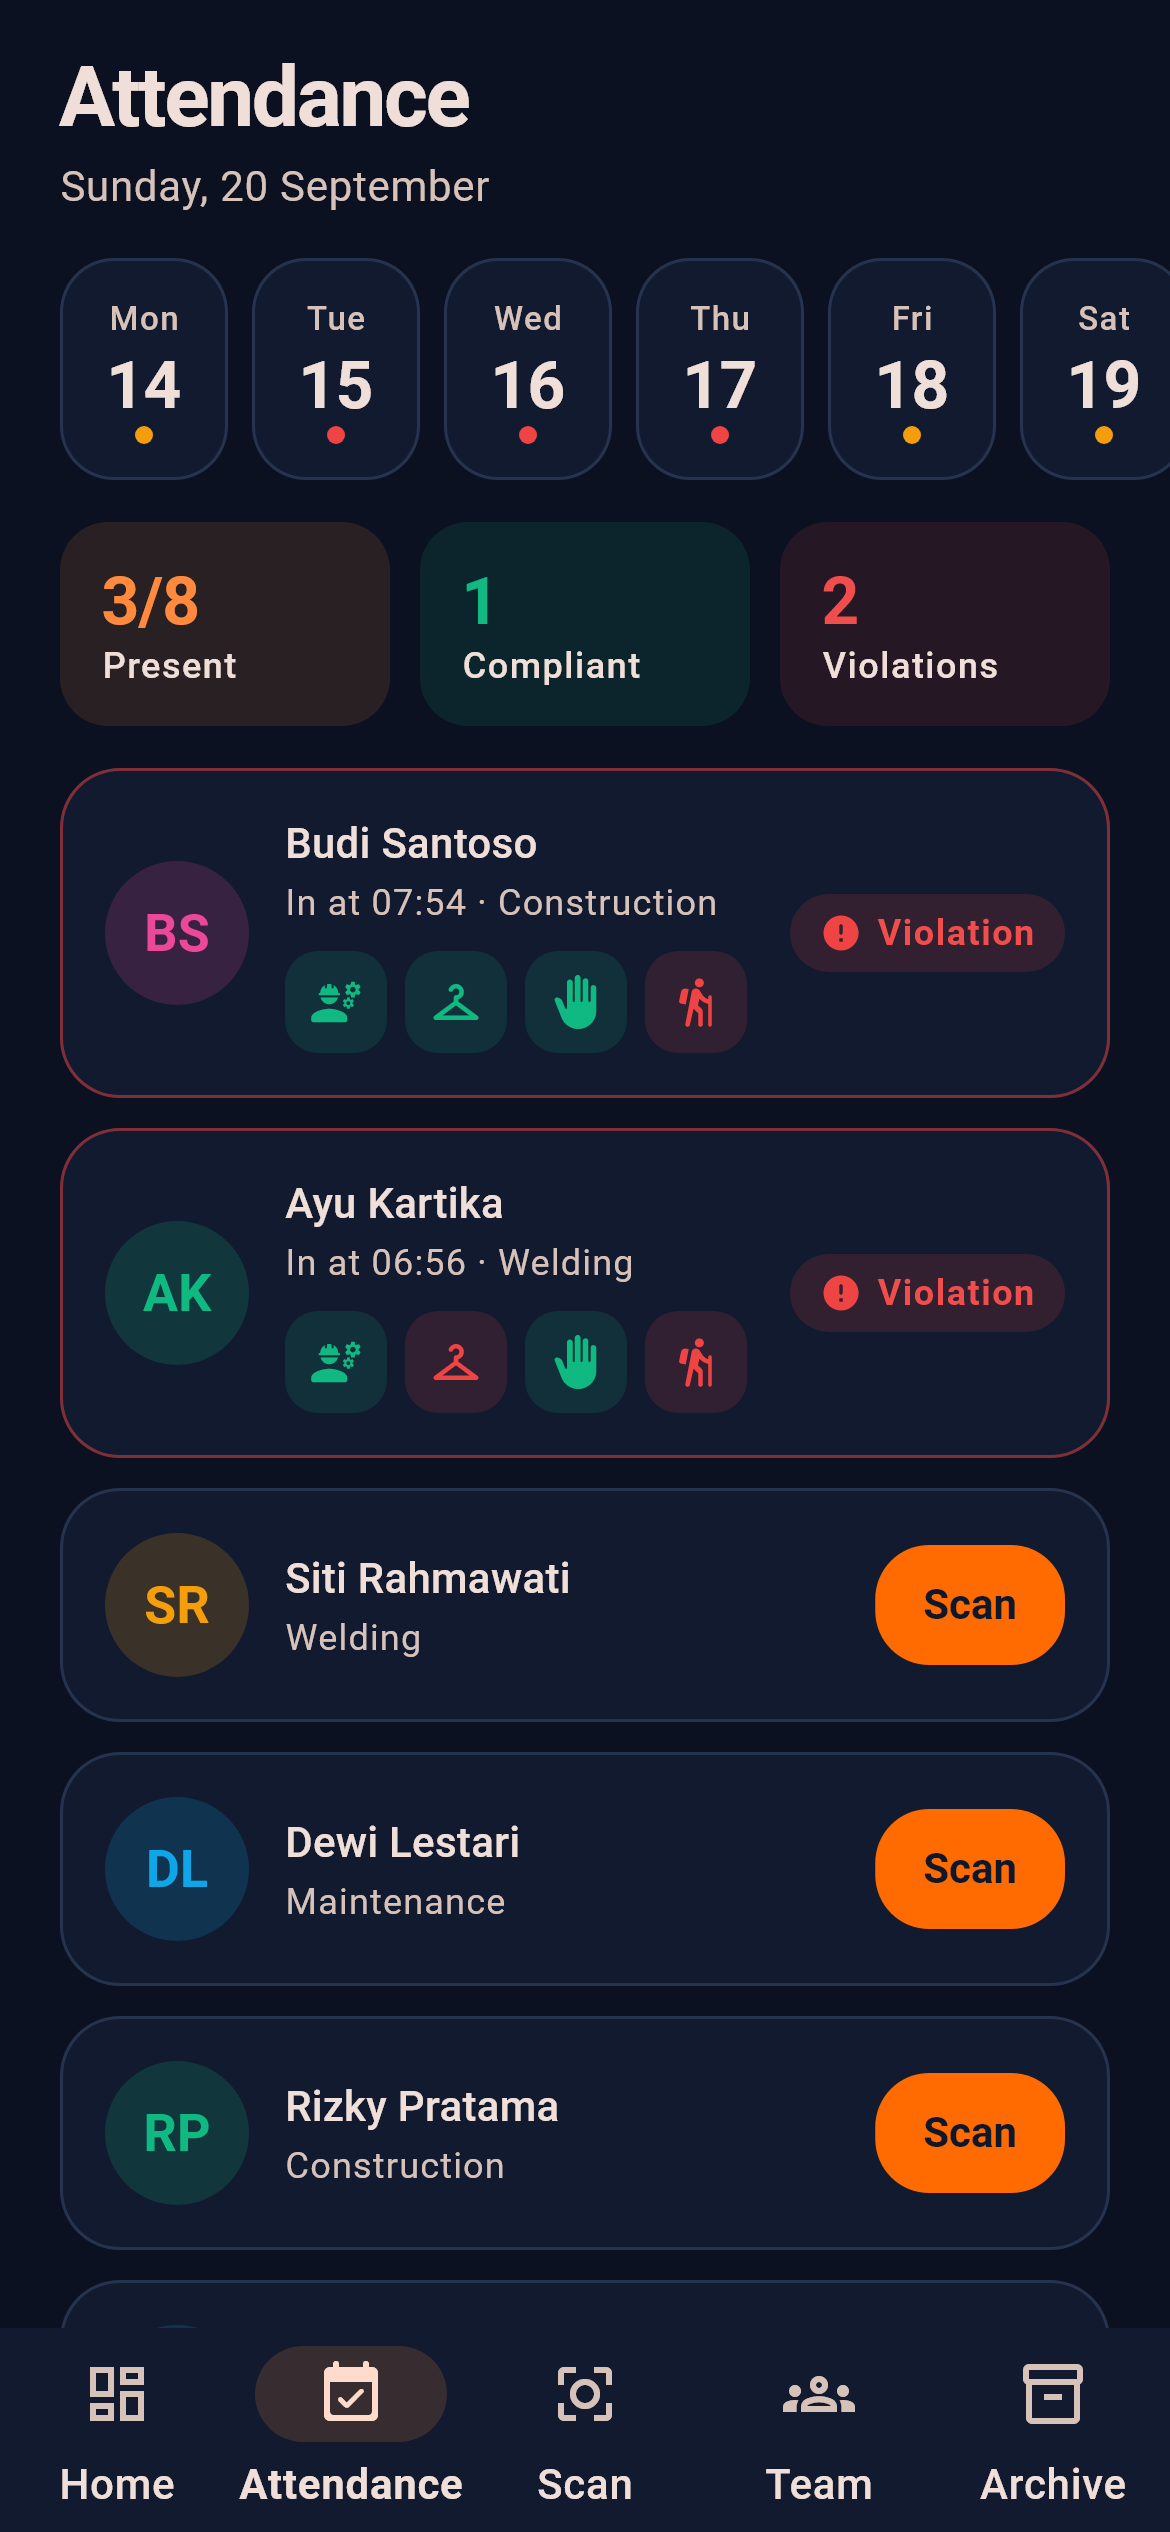
\includegraphics[width=0.42\columnwidth]{05-attendance.png}
\caption{Scan result with per-item confidence (left) and attendance view (right).}
\label{fig:scan}
\end{figure}

\subsection{Persistence and Reporting}
Employees and scans are stored as versioned JSON in platform key--value
storage, which works on mobile, desktop and web. A report generator produces a
branded A4 PDF containing summary indicators and a per-scan table for a single
scan, one worker, or the current archive filter.

\section{Implementation and Verification}
The implementation targets Flutter 3.41 / Dart 3.11 and comprises 32 source
files (about 4.9k lines) and Android, iOS, web, Windows and macOS runners.
\subsection{Static Analysis and Tests}
The project passes \texttt{flutter analyze} with no errors or warnings under
the \texttt{very\_good\_analysis} rule set (two informational lints remain).
The test suite has seven tests: three unit tests (compliance maths and JSON
round-trip, deterministic seed data, detector output range) and four
end-to-end widget tests (onboarding gate; running a scan and saving a
violation; adding an employee; filtering the archive).
\subsection{Detector Used in the Current Build}
\textbf{The current build uses a simulated detector} that draws item
confidences at random after a short delay. It exists to exercise the complete
workflow without a camera or trained model; consequently \emph{no detection
accuracy is claimed in this paper}.

\section{Evaluation}
\todo{Replace this section with real experiments before submission. Minimum
recommended content:}
\subsection{Detector Benchmark}
\todo{Train/evaluate a real PPE detector (state dataset, split, hyper-parameters,
hardware). Report precision, recall, mAP@0.5 and mAP@0.5:0.95 per class, and
on-device latency (ms/frame) and memory on named phones.}
\subsection{Usability Study}
\todo{Recruit $n$ supervisors or representative users; use task-completion time
and success rate for the core tasks (scan, find a violation, export a report),
plus the System Usability Scale~\cite{brooke1996}. Report mean, SD and the
protocol; obtain ethics approval or an exemption statement.}
\subsection{Ablation of the Workflow}
\todo{Compare time-to-record with a paper checklist baseline.}

\section{Discussion and Limitations}
Compliance is decided per item from a single frame; occlusion, lighting and
multiple workers per frame are not modelled. Worker identity is chosen from a
list rather than recognised automatically. Storage is local to the device.
Camera-based monitoring of people raises privacy and labour-consent issues; a
deployment must define retention and consent policies and should store scores
rather than images. \todo{Discuss applicable regulation for the target country.}

\section{Conclusion}
We presented GearGuard, a detector-agnostic architecture and open-source
implementation of the PPE compliance workflow. Future work is a real on-device
detector behind the same interface, a field usability study, and
department-level reporting.

\section*{Acknowledgment}
\todo{Funding, supervisors, data providers.}

\bibliographystyle{IEEEtran}
\bibliography{refs}

\end{document}
